% Drawing 142/02-8 -- folder 142, batch 02, archive page 32 (PDF page 33).
% Transcription: sphère réunissant les figures précédentes : pôles $P^{+}$, $P^{-}$ ; sur l'équateur, $Q_0$, $Q_1$, $Q_\infty$ et, autour de chacun des trois points marqués, le petit cercle $R_i^{\pm}$ avec les arcs $a_i^{\pm}$ ; les arcs $c_i^{\pm}$ joignant les $Q$ aux $R$, et les méridiens $d_i^{\pm}$. Légende : $\mathrm{VI}$.
% Kind: sphere with poles, meridians, equatorial vertices and small circles. Method 2 (schematic redraw from the facsimile). Status: partial.
% Notes: Pencil outline; P^+ and P^-; meridians d_0^+- solid from the poles to Q_0, d_infty^+- and d_1^+- dashed from the poles to Q_infty and Q_1 (the hidden d_1^- passing behind the circle round infinity), each with its arrow into the Q; Q_infty, Q_0, Q_1; the three small circles round the marked points, dotted round 0 (top middle), solid round 1 (left) and round infinity (right), each with its two points R^+- on it and its two arcs a^+ (upper half) and a^- (lower half); the arrows c from the Q to the R, each ending at the same R point as its circle: c_infty^- (dashed) from Q_infty to R_0^+, c_infty^+ from Q_infty round the left to R_1^-, c_1^+ (dotted) from Q_1 to R_0^-, c_0^- from Q_0 to R_1^+, c_0^+ from Q_0 to R_infty^-, and the dotted stroke from Q_1 that runs off the right edge (towards R_infty^+, whose label is cut). Still differs: the small arrowheads on the circles are not drawn; the stroke from Q_1 to the right is cut by the edge of the crop; his doubled pencil strokes at the bottom left and bottom right are reduced to one, and the wavy hatching near P^- is not drawn; the small mark above d_infty^+ is left out. Nothing is struck. Redrawn 2026-11-09 (issue 128): to check again.
% Coordinates: 1 unit = 1 mm = 1/100 of the crop width (bbox in page fractions: [0.12, 0.1, 0.5, 0.38]).
% Redrawn by Claude (claude-opus-5-5), issue #73, 2026-11-09; not checked by a human; not compiled (no TeX in the session).
% Rights: reproduces part of the work -- behind RENDER_TRANSCRIPTS, never published by itself.
\documentclass[tikz,border=3pt]{standalone}
\usepackage{amsmath,amssymb}
\usetikzlibrary{patterns,arrows.meta}
\tikzset{pencil/.style={black!45}, struck/.style={black!35}, mark/.style={circle,draw,inner sep=1.3pt}, pt/.style={circle,fill,inner sep=0.9pt}, opt/.style={circle,draw,fill=white,inner sep=1.1pt}}
\begin{document}
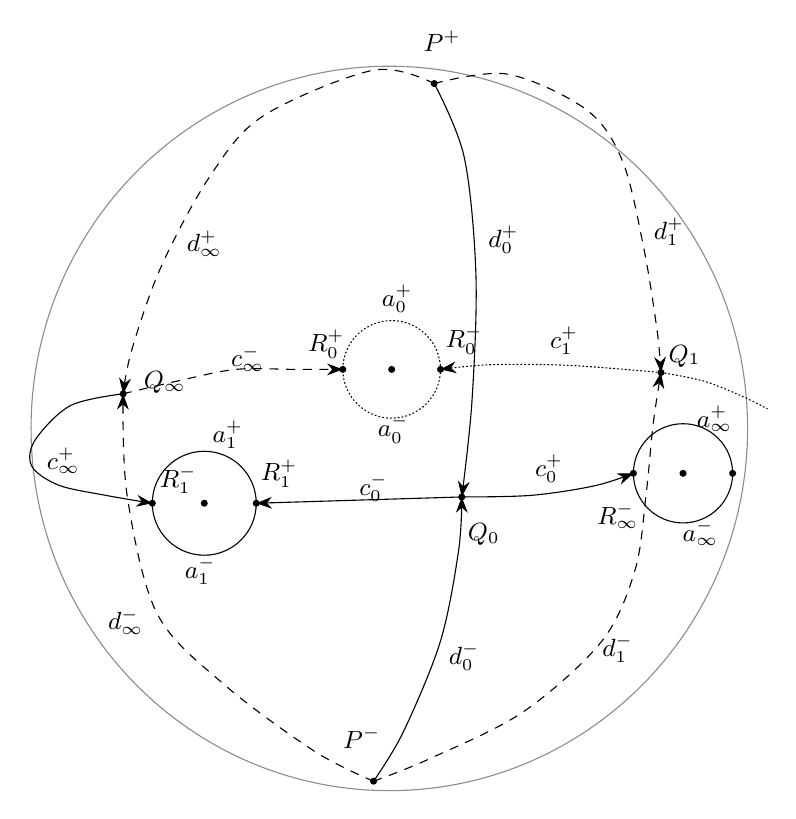
\begin{tikzpicture}[x=1mm,y=1mm,line cap=round,line join=round,font=\scriptsize]
\draw[pencil] (52,-57.5) ellipse[x radius=45.5, y radius=46];
\node[pt] at (57.7,-13.7) {};
\node[pt] at (50,-102.3) {};
\node[pt] at (18.2,-53.1) {};
\node[pt] at (61.2,-66.2) {};
\node[pt] at (86.5,-50.4) {};
\node[pt] at (46.1,-50) {};
\node[pt] at (58.5,-50) {};
\node[pt] at (21.9,-67) {};
\node[pt] at (35.1,-67) {};
\node[pt] at (83,-63.2) {};
\node[pt] at (95.6,-63.2) {};
\node[pt] at (52.3,-50) {};
\node[pt] at (28.5,-67) {};
\node[pt] at (89.3,-63.2) {};
\draw[densely dotted] (52.3,-50) circle[radius=6.2];
\draw (28.5,-67) circle[radius=6.6];
\draw (89.3,-63.2) circle[radius=6.3];
\draw[-{Stealth[length=2mm]}] plot[smooth, tension=0.55] coordinates {(57.7,-13.7) (61.5,-23) (63,-38) (62.5,-54) (61.2,-66.2)};
\draw[-{Stealth[length=2mm]}] plot[smooth, tension=0.55] coordinates {(50,-102.3) (53.8,-96) (58.5,-84.5) (60.8,-73) (61.2,-66.2)};
\draw[dashed,-{Stealth[length=2mm]}] plot[smooth, tension=0.55] coordinates {(57.7,-13.7) (50,-12) (36,-17.8) (29.2,-25.5) (23,-37) (19.3,-47.5) (18.2,-53.1)};
\draw[dashed,-{Stealth[length=2mm]}] plot[smooth, tension=0.55] coordinates {(50,-102.3) (42.5,-98.5) (31,-90) (22.5,-81) (18.7,-66) (18.2,-53.1)};
\draw[dashed,-{Stealth[length=2mm]}] plot[smooth, tension=0.55] coordinates {(57.7,-13.7) (67,-12.5) (77,-17) (81.6,-23.5) (84.3,-34.5) (86,-45) (86.5,-50.4)};
\draw[dashed,-{Stealth[length=2mm]}] plot[smooth, tension=0.55] coordinates {(50,-102.3) (57,-99.5) (69,-93.5) (79,-84.5) (83.2,-75.5) (84.6,-66) (85.5,-57) (86.5,-50.4)};
\draw[dashed,-{Stealth[length=2mm]}] plot[smooth, tension=0.55] coordinates {(18.2,-53.1) (25,-51.5) (32.5,-50) (40,-50) (46.1,-50)};
\draw[-{Stealth[length=2mm]}] plot[smooth, tension=0.55] coordinates {(18.2,-53.1) (11.5,-54.6) (7,-59) (6.6,-62.3) (10,-64.7) (16,-66) (21.9,-67)};
\draw[densely dotted,-{Stealth[length=2mm]}] plot[smooth, tension=0.55] coordinates {(86.5,-50.4) (75,-49.5) (65,-49.4) (58.5,-50)};
\draw[-{Stealth[length=2mm]}] (61.2,-66.2) -- (35.1,-67);
\draw[-{Stealth[length=2mm]}] plot[smooth, tension=0.55] coordinates {(61.2,-66.2) (70,-66) (78,-64.8) (83,-63.2)};
\draw[densely dotted] plot[smooth, tension=0.55] coordinates {(86.5,-50.4) (92,-51.5) (97,-53.5) (100,-55)};
\node[inner sep=1pt] at (58.7,-8.3) {\small $P^{+}$};
\node[inner sep=1pt] at (48.5,-96.8) {\small $P^{-}$};
\node[inner sep=1pt] at (23.5,-51.7) {\small $Q_\infty$};
\node[inner sep=1pt] at (64,-71) {\small $Q_0$};
\node[inner sep=1pt] at (89.5,-48.3) {\small $Q_1$};
\node[inner sep=1pt] at (28.5,-34) {\small $d_\infty^{+}$};
\node[inner sep=1pt] at (66.5,-33.5) {\small $d_0^{+}$};
\node[inner sep=1pt] at (87.5,-32.5) {\small $d_1^{+}$};
\node[inner sep=1pt] at (18.5,-82) {\small $d_\infty^{-}$};
\node[inner sep=1pt] at (61.5,-86.5) {\small $d_0^{-}$};
\node[inner sep=1pt] at (81,-85.5) {\small $d_1^{-}$};
\node[inner sep=1pt] at (34,-48.6) {\small $c_\infty^{-}$};
\node[inner sep=1pt] at (10.6,-61.6) {\small $c_\infty^{+}$};
\node[inner sep=1pt] at (74.2,-46.4) {\small $c_1^{+}$};
\node[inner sep=1pt] at (50,-65) {\small $c_0^{-}$};
\node[inner sep=1pt] at (72.3,-62.6) {\small $c_0^{+}$};
\node[inner sep=1pt] at (53,-41) {\small $a_0^{+}$};
\node[inner sep=1pt] at (52.5,-57.6) {\small $a_0^{-}$};
\node[inner sep=1pt] at (31.5,-58.3) {\small $a_1^{+}$};
\node[inner sep=1pt] at (28,-75.6) {\small $a_1^{-}$};
\node[inner sep=1pt] at (93.3,-56.3) {\small $a_\infty^{+}$};
\node[inner sep=1pt] at (91.5,-70.8) {\small $a_\infty^{-}$};
\node[inner sep=1pt] at (44,-46.8) {\small $R_0^{+}$};
\node[inner sep=1pt] at (61.5,-46.3) {\small $R_0^{-}$};
\node[inner sep=1pt] at (25.2,-64) {\small $R_1^{-}$};
\node[inner sep=1pt] at (38,-63.2) {\small $R_1^{+}$};
\node[inner sep=1pt] at (81,-68.6) {\small $R_\infty^{-}$};
\end{tikzpicture}
\end{document}
